\documentclass[a4paper,12pt]{article}
%\documentclass[a4paper,10pt]{scrartcl}

\usepackage[margin=0.8in]{geometry}
\usepackage[utf8]{inputenc}
\usepackage{graphicx}

\title{Synchronization of Lines in an Image}
\author{Bnumeros\_Report1}
\date{\today}



\begin{document}
\maketitle

\begin{abstract}
 This report outlines a proposed procedure for synchronising lines of an image that has been corrupted by randomly shifting horizontal lines. The method involves the use of discrete fourier transforms of each line in the given image to determine to what degree each of them was shifted. The end result of the procedure is an image that has been reconstructed to an almost perfect extent, with the edges of the output images being the most notorious unfixed problem.
\end{abstract}

\section{Introduction}

The field of digital image processing aims to modify images through the use of various mathematical operations. This is done by considering images as two dimensional objects and applying signal processing techniques to them in order to manipulate them~\cite{gonzalez1992digital}. This work describes an algorithm that uses image processing techniques to synchronise an image. In this particular case, said input image has had certain horizontal lines randomly shifted. The input corrupted image must be in file format \texttt{.pgm} (Portable Graymap), since this file format can be read as a two dimensional array, for example fig.~\ref{fig.1}. After passing the input image through the devised algorithm, the output should have most lines shifted into their appropriate location. Some information is lost in the output image - this occurs mainly in the image's edges, this will be elaborated in the next section.

\begin{figure}[h!]
\centering
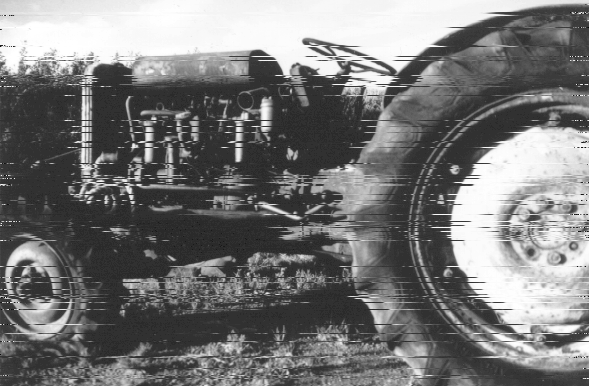
\includegraphics[width=0.73\textwidth]{img/desync2}
\caption{Randomly shifted horizontal lines.}
\label{fig.1}
\end{figure}

The algorithm used to attempt to synchronise the horizontal lines of the given images was written in Python3.5, and imports the libraries: \texttt{os} for handling the input and output of images (hopefully) without errors, \texttt{matplotlib.pyplot} for showing the enhanced image (which is then optionally saved by the user), \texttt{misc} from \texttt{scipy} to read the \texttt{.pgm} input files and write the output file, and \texttt{numpy} since it allows for the use of Discrete Fourier Transform (DFT, which are a fundamental component of the algorithm). Version control was implemented in the development of the algorithm. Consequently, the code is available in a public \texttt{github} repository under the following url: \texttt{https://github.com/quietF/NumRep} on the folder \texttt{FT}. There, a short \texttt{README} file details the implementation of the code. Nevertheless, the code is also included in an annex in the end of this report. 

In broad terms, which will be elaborated on later on, the algorithm takes the two dimensional image and compares vertically adjacent lines by calculating the cross correlation between them. From this, the number of pixels that these lines have been shifted is obtained. This allows for a reconstruction of the image. Some limiting cases must be considered to get the enhanced image. It must be said that the developed algorithm can be improved since not all images are perfectly reconstructed. The following sections will elaborate on this. 

\section{Aim and Methods}

The aim of this problem is to take an image in grayscale format with an arbitrary number of horizontally shifted lines and attempt to place them in their right position. Since the line desynchronisation is exclusive to the horizontal direction, i.e. no lines have a vertical shift, it is sensible to divide the two dimensional image into a series of one dimensional objects, where each object is a horizontal line. 

Through the use of various mathematical methods it is possible to find the degree to which each horizontal line has been shifted. The method described, and used, relies on a very strong assumption - vertically adjacent lines can be considered as being approximately equal. This is justified by the fact that most lines in the input images will indeed be very similar. For example, lines \#0 and \#1 from one of the images are plotted as a signal in fig.~\ref{fig.2} and~\ref{fig.3}. This, however, will not always be true, and will lead to problems in the algorithm. Since the one dimensional objects, horizontal lines, are being treated as signals, it is adequate to look for signal processing tools to find how to synchronise the lines. An operation that compares two signals for their similarity is necessary. This is precisely the cross correlation of two functions.

\begin{figure}[h]
\centering
\begin{minipage}{.5\textwidth}
  \centering
  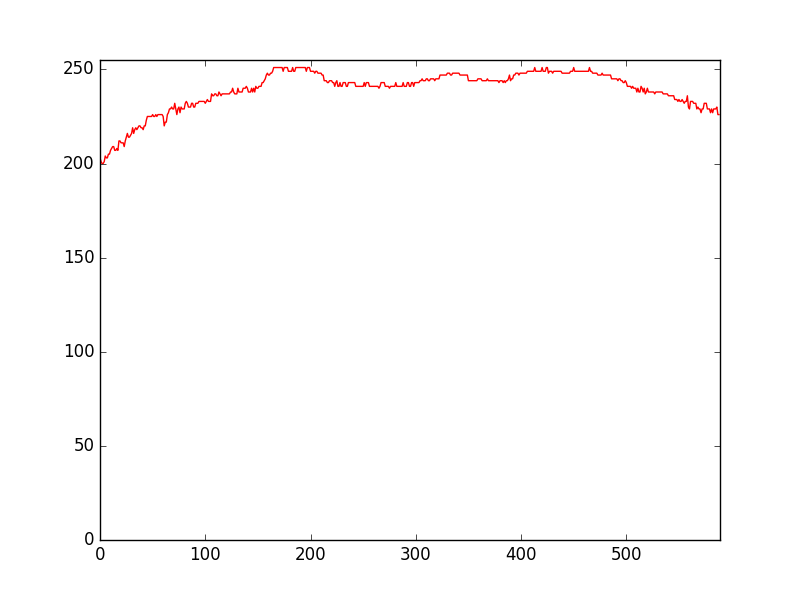
\includegraphics[width=1.05\linewidth]{img/line0}
  \caption{Horizontal line \#0 from the top.}
  \label{fig.2}
\end{minipage}%
\begin{minipage}{.5\textwidth}
  \centering
  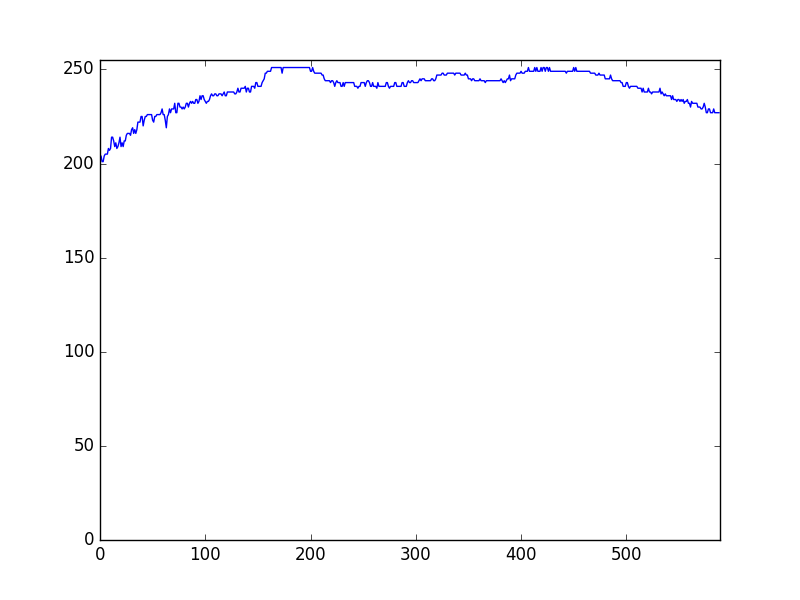
\includegraphics[width=1.05\linewidth]{img/line1}
  \caption{Horizontal line \#1 from the top.}
  \label{fig.3}
\end{minipage}
\end{figure}

If two signals are defined by functions $f(t)$ and $g(t)$, then the cross correlation between the two signals is defined as eqn.~\ref{eq.1}, where the notation for complex conjugate is $f^*$, as usual~\cite{bracewell2012fourier}.  

\begin{equation}
 (f \star g)(\tau) = \int_{-\infty}^{\infty} f^*(t) g(t+\tau) dt
 \label{eq.1}
\end{equation}

This can be expressed in a much more simple fashion, by making use of the properties of the Fourier Transforms. Doing so results in a much more simple expression for the cross correlation between two signals. This expression is shown in eqn.~\ref{eq.2}, where $\mathcal{F}\{ f \}$ denotes the Fourier Transform of the signal $f$~\cite{bracewell2012fourier}.

\begin{equation}
 \mathcal{F}\{ f \star g \}(\tau) = (\mathcal{F}\{ f \})^* \cdot \mathcal{F}\{ g \}
 \label{eq.2}
\end{equation}

This means that if the Fourier Transform of each line can be obtained, then retrieving the cross correlation between lines is simply a multiplication, followed by an Inverse Fourier Transform. Luckily, the scientific computing package available for Python, \texttt{numpy}, has a simple way of obtaining the Discrete Fourier Transform (DFT) of an array (as well as its Inverse DFT). These are all methods under the routine \texttt{numpy.fft} (which stands for ``fast Fourier Transform''). Figure~\ref{fig.4} shows exactly this by taking the normalised cross correlation of both signals in fig.~\ref{fig.2} and~\ref{fig.3}. 

\begin{figure}[h!]
\centering
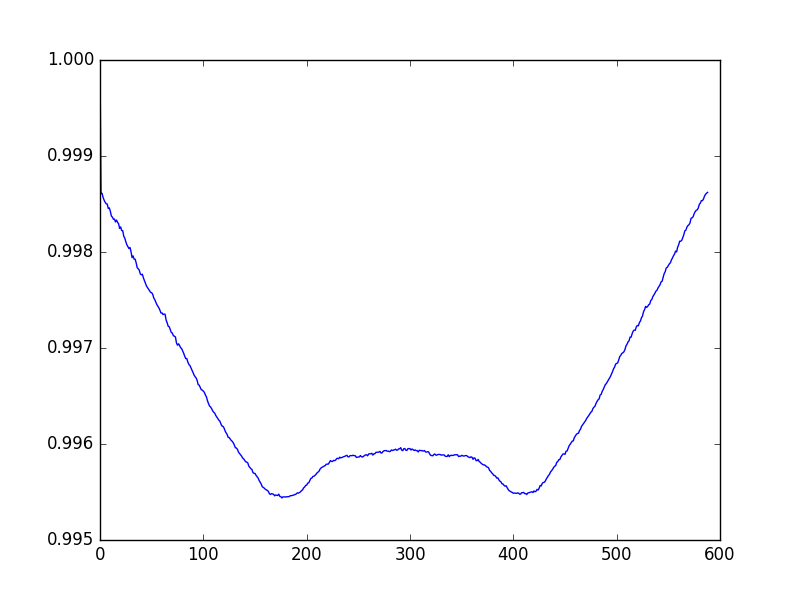
\includegraphics[width=0.73\textwidth]{img/xcorrelation}
\caption{Cross correlation of fig.~\ref{fig.2} and~\ref{fig.3}.}
\label{fig.4}
\end{figure}

The maximum of the cross correlation is located at 0 in the x axis. This means that no shift needs to be made in order to maintain the two images as the ``same''. When this maximum is not located at 0, then it is likely that a shift needs to be made in order to synchronise those lines. From this a basic idea of what the algorithm has to be can be devised. The process would be something along these lines: 

\begin{enumerate}
 \item Obtain the DFT of line \#i and of line \#i-1.
 \item Obtain the normalised cross correlation of the two DFTs.
 \item Shift line\#i such that the cross correlation maximum is located at 0.
\end{enumerate}

Following said method for all lines (excluding line \#0 as it has no line above to compare) should reconstruct the image to its right position. The result for fig.~\ref{fig.1} after going through the method described is shown in fig.~\ref{fig.5}. Clearly something has gone wrong and the shift has been too careless, but not everything is bad. Other than the edges, the image has been reconstructed to an acceptable extent. However, this can be improved.

\begin{figure}[h!]
\centering
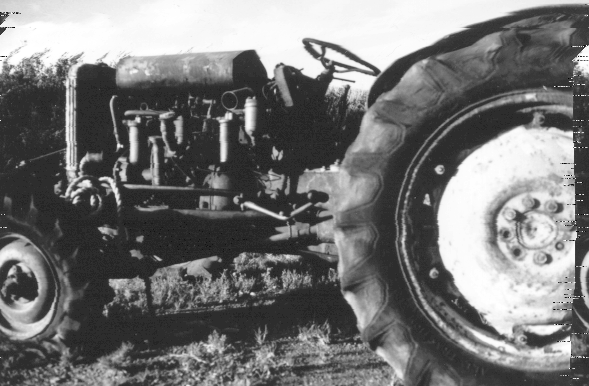
\includegraphics[width=0.73\textwidth]{img/simple}
\caption{First synchronising method for fig.~\ref{fig.1}.}
\label{fig.5}
\end{figure}

\newpage

\bibliographystyle{unsrt}
\bibliography{report1}

\end{document}
